\documentclass[11pt]{article}
\usepackage{graphicx}
\usepackage[colorlinks,linkcolor=blue]{hyperref}

\title{Homework 6}
\date{\today}
\author{Zhiyuan Hu}
\begin{document}
	\maketitle
	\section{Task Introduction}
	\subsection{The data:}
	\begin{itemize}
		\item Input is a sequece of binary number, time t, input is 0 or 1, both are 50\% probability. Like $X = [1,1,0,0,1,.....]$.
		\item 
		Output Y at time t is also 0 or 1 with 50\% probability. But if $X_{t-3}=1$, probability of $Y_t = 1$ increase 50\%. if $X_{t-8}$ is 1, probability of $Y_t = 1$ decreases 25\%.
	\end{itemize}
	\subsection{Loss:}
	Use cross entropy to train the function.
	\subsection{Reference:}
	Code Link is here. \href{ https://github.com/lawlite19/Blog-Back-Up/blob/master/code/rnn/rnn_implement.py}{Github Link}\\ 
	Paper Link \href{https://r2rt.com/recurrent-neural-networks-in-tensorflow-i.html}{here}
	 \href{https://r2rt.com/styles-of-truncated-backpropagation.html}{here} \href{https://web.stanford.edu/class/psych209a/ReadingsByDate/02_25/Williams%20Zipser95RecNets.pdf}{here}
\section{Network}
	Like as is shown in the figure1 and figure 2:\\
\begin{figure}[htbp]	
	\centering
	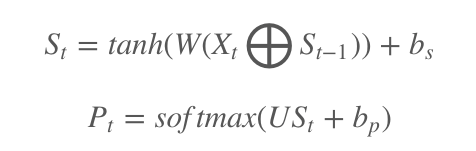
\includegraphics[width=0.5\linewidth]{pic/111}
	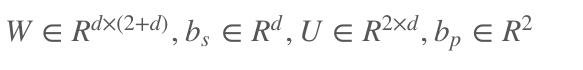
\includegraphics[width=0.5\linewidth]{pic/222}
	\caption{}
\label{fig:111}
\end{figure}
\begin{figure}[htbp]	
	\centering
	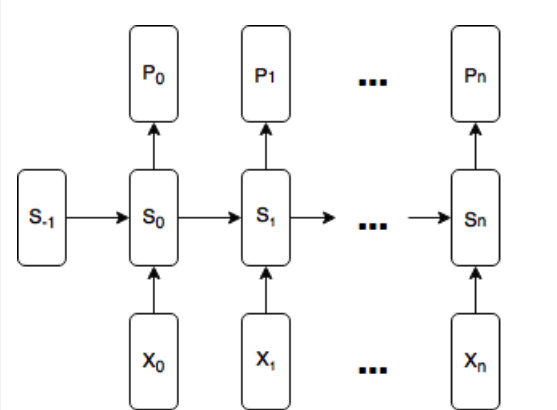
\includegraphics[width=0.5\linewidth]{pic/333}
	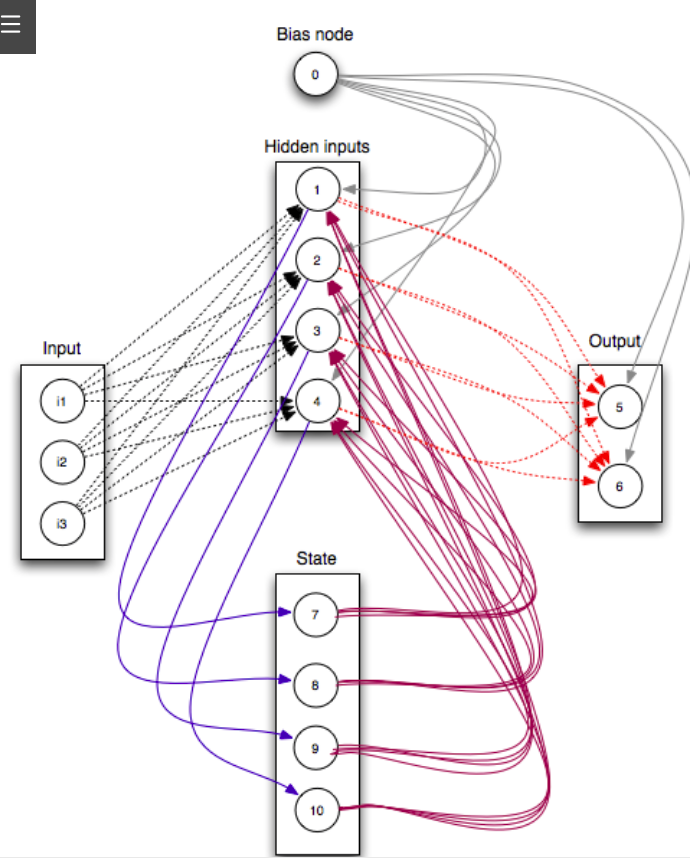
\includegraphics[width=0.5\linewidth]{pic/444}
	\caption{}
	\label{fig:333}
\end{figure}
\section{Implementation in Tensorflow}
Justlike as is shown in figure 3:
\begin{figure}
	\centering
	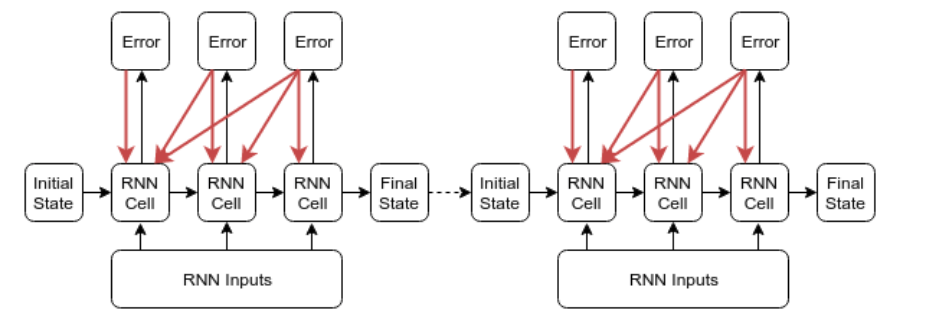
\includegraphics[width=0.9\linewidth]{pic/555}
	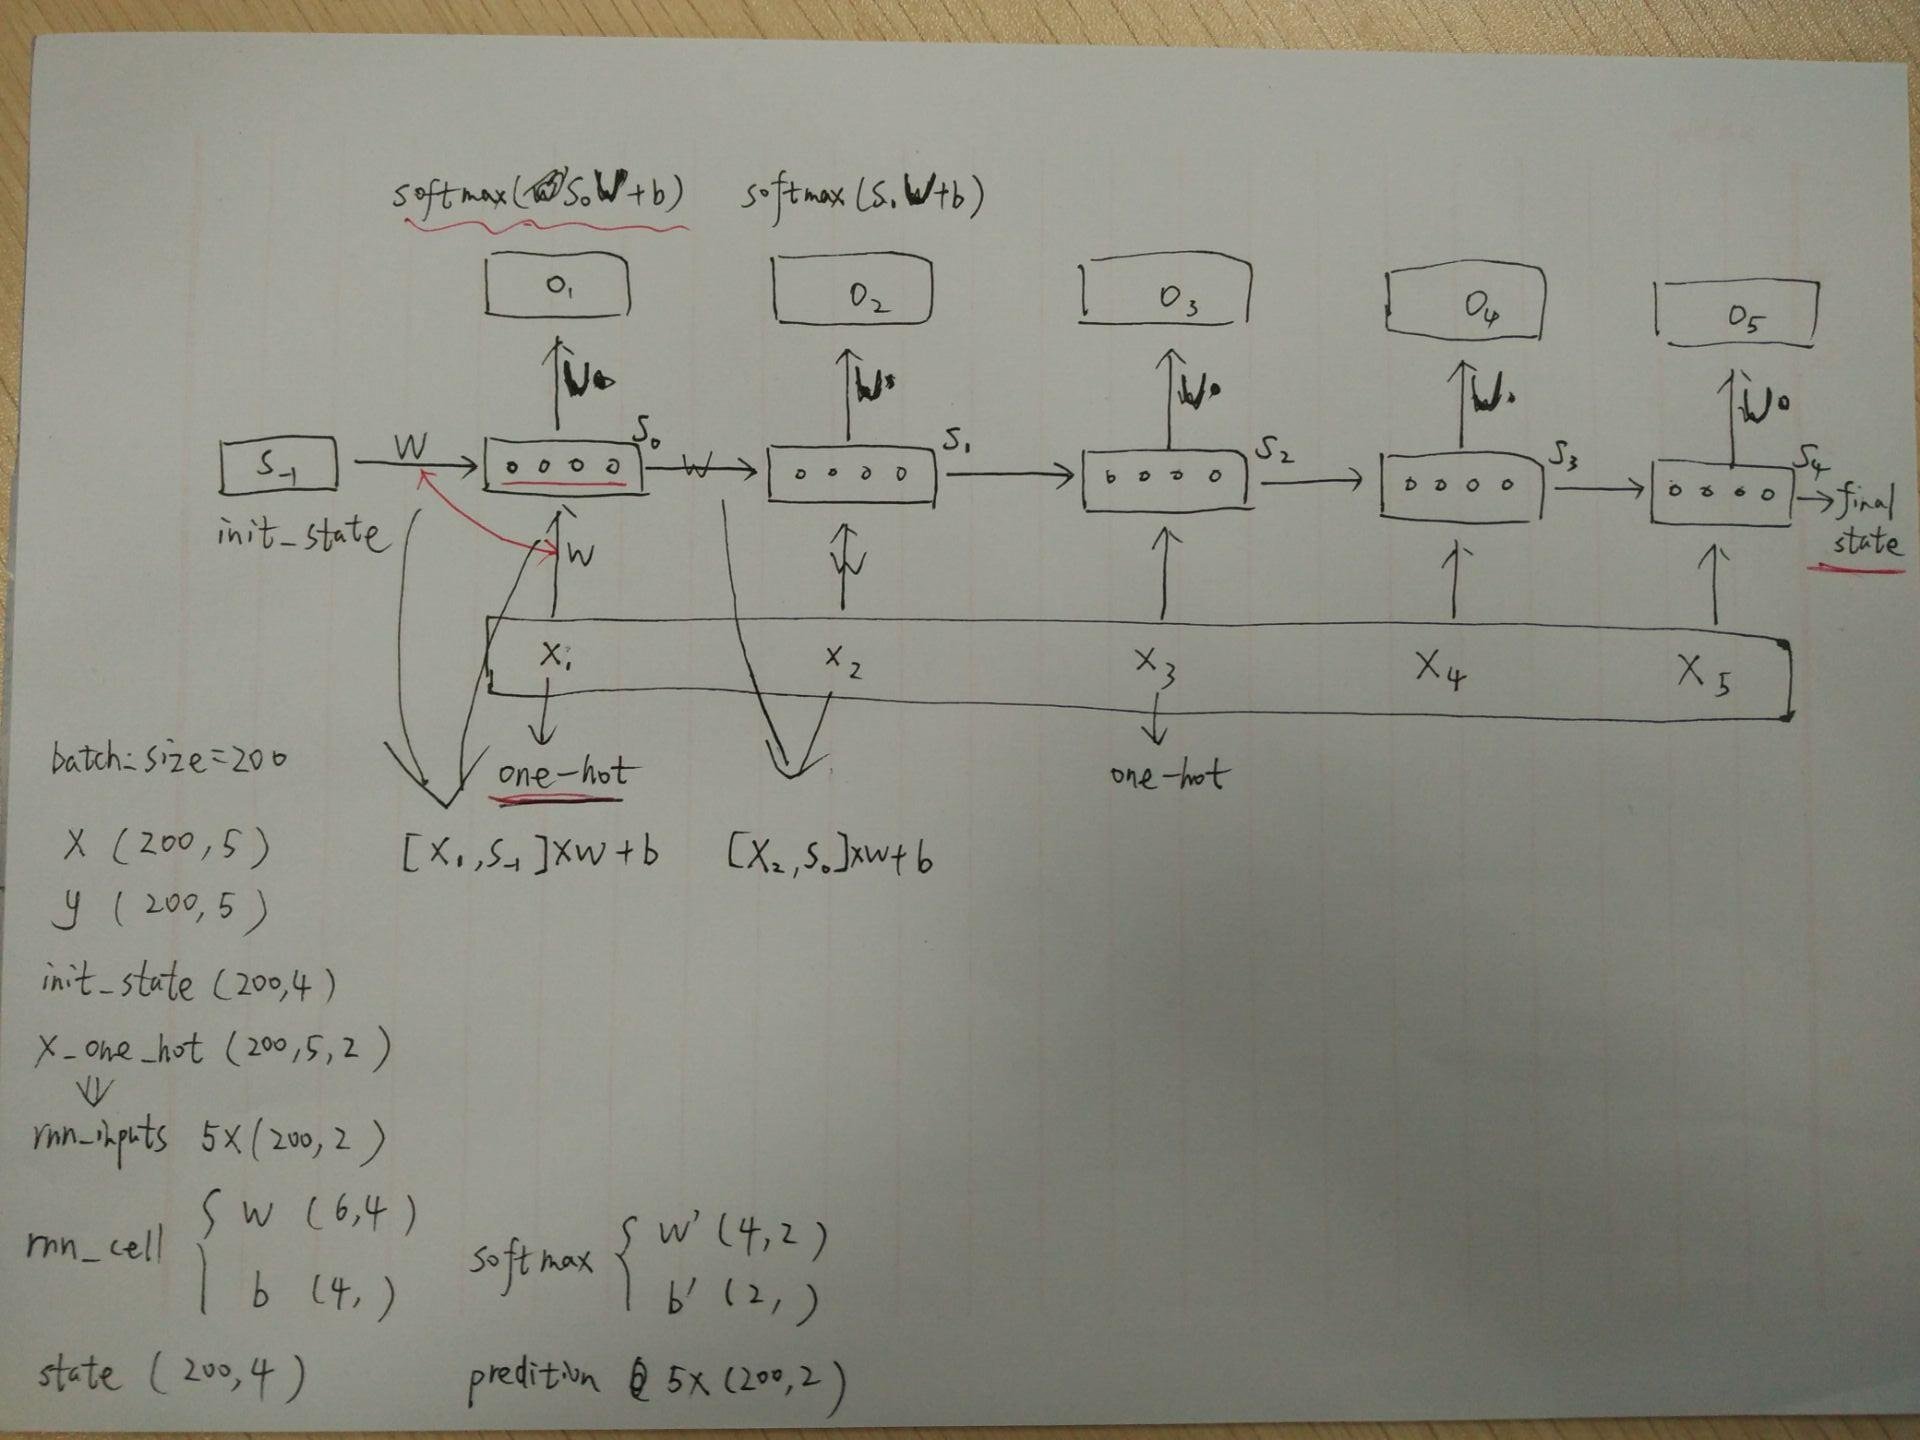
\includegraphics[width=0.9\linewidth]{pic/RNN_14}
	\caption{}
	\label{fig:555}
\end{figure}
\section{Result}
Like as is shown in figure 4. with num\_step 10 and state 16, finally the network has learned the dependencies and loss is nearby 0.45.
\begin{figure}
	\centering
	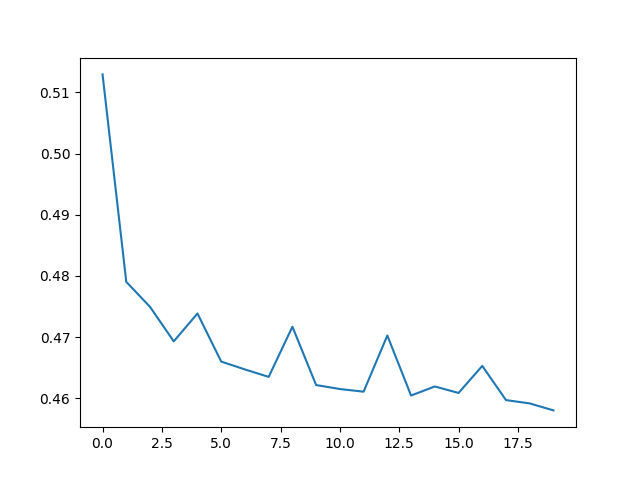
\includegraphics[width=0.7\linewidth]{pic/RNN_15}
	\caption{}
	\label{fig:rnn15}
\end{figure}


\end{document}